\documentclass[conference, 11pt]{IEEEtran}
\usepackage[style=ieee]{biblatex}
\usepackage[english]{babel}
\usepackage{csquotes}
\usepackage[nottoc]{tocbibind}
\usepackage{graphicx}
\usepackage{nameref}
\usepackage[hidelinks]{hyperref}
\usepackage{sidecap}
\usepackage{wrapfig}
\usepackage[bottom,hang]{footmisc} 
\usepackage{acronym}
\usepackage{color}
\usepackage{afterpage,hyperref} 
\usepackage{listings}
\usepackage{subfigure}
\usepackage{array,			%better tables
			tabularx,			    %instead of tabular*             
			booktabs,			%tables for good publications
}

\addbibresource{literature_list.bib}
\renewcommand*{\bibfont}{\small}

\begin{document}
\title{The Protection of Bystanders' Privacy\\Seminar on Privacy in Ubiquitous Computing}

\author{\IEEEauthorblockN{Mehmed Mustafa}
\IEEEauthorblockA{\textit{Institute of Computer Science} \\
\textit{University of Göttingen}\\
mehmed.mustafa@stud.uni-goettingen.de}
\and
\IEEEauthorblockN{Chris Warin} 
\IEEEauthorblockA{\textit{Institute of Computer Science} \\
\textit{University of Göttingen}\\
chris.warin@stud.uni-goettingen.de
}
}

\maketitle
\thispagestyle{plain} %--to make title page number less
\pagestyle{plain}    % -- to make other pages number less.

\begin{abstract}
The ubiquitous presence of privacy-threatening devices in nowadays' society is an issue that touches several domains, including economic, social, legal and technological. In this report, we present an overview of the situation regarding the privacy of bystanders, a topic that is getting more attention in research due to rising concerns. We describe the nature of devices that can threaten the visual, audio, and location privacy of bystanders in various situations: they include smartphones, drones, and, more recently, \ac{IoT} devices such as smart-home devices. We then discuss over a number of past attempts at solutions that were unfruitful, before coming to our focus by presenting three technologies that aim to protect the privacy of bystanders. We denote two major approaches: one that takes action upon the collection of data (e.g. visual abstraction of bystanders when they are being photographed), one upon the online-sharing of interdependent data. The technologies adopting the former approach rely on user participation: bystanders register a privacy profile that is accessed by the system when it recognizes them. This gives a necessary flexibility to those systems, because of the different requirements regarding privacy across different individuals. The latter approach is perhaps even more crucial, as the sharing of interdependent data without the knowledge or the consent of the implied bystanders can have disastrous consequences. The limitations and challenges of the presented technologies are also discussed; the main challenge being the inclusion of such systems in everyday's life apps and websites, to efficiently start protecting bystanders' privacy.
\end{abstract}

\begin{IEEEkeywords}
privacy, bystander, privacy enhancing technology
\end{IEEEkeywords}

\section{Introduction}\label{Intro}
Today's society is filled with technological devices that are capable of gathering data from people, such as smartphones, surveillance cameras, \ac{AR} devices or \ac{IoT} devices \cite{lu2017privacy, shu2016cardea, denning2014situ}. Although these devices have been causing a number of concerns regarding the privacy of users, recent studies have shown that the privacy of bystanders (i.e. the individuals that are around users using these devices) is also often involved, as online-shared data often involves individuals other than the users sharing the data~\cite{olteanu2018consensual}. In other words, bystanders' personal information can be collected without their knowledge or consent~\cite{lu2017privacy}. This, along with the high amount of devices capable of collecting data of different nature, results in high pervasiveness in bystanders' privacy, which has increased people's concerns about their visual privacy. Even when taking photos is not involved, applications making use of the camera, such as \ac{AR} apps, could still compromise the visual privacy of bystanders by leaking the captured visuals, maliciously or not. This is a significantly harder problem to solve than regular user privacy, mainly because bystanders can be unaware that data involving them is shared in the first place~\cite{olteanu2018consensual}.

%Past attempts
In the past, several attempts with different approaches have been made in order to ensure the privacy of bystanders. Technological solutions exist to protect the\textemdash mainly\textemdash visual privacy of bystanders, which can be compromised in many different cases. Regarding video surveillance systems, the authors of \cite{chinomi2008PriSurv} point out that their high deployment rate in public places leads to privacy invasion of the objects (i.e. individuals) being recorded, which motivated a number of studies. Two studies proposed image processing methods in order to protect the privacy of objects \cite{cavallaro2005, kitahara2004}. In two other studies, the privacy protection of objects depends either on the authority of objects or observers \cite{jehan2005, senior2005}. Privacy information can be embedded by using digital watermarking technology in such way that only predefined authorized viewers will have access to it \cite{zhang2005}. Later, there were proposals for using visual markers \cite{roesner2014, liu2014} or colourful hats \cite{sastry2007} with which people can declare their disagreement to be captured. These approaches, however, are not flexible enough, because people should be able to control, modify and express their individual privacy preferences naturally\textemdash without the need of any extra facilities. 

On the online-sharing side, Olteanu, Huguenin, Dacosta and Hubau \cite{olteanu2018consensual} claim that few solutions exist for detecting and sharing interdependent data in a way that preserves privacy of interdependent users. They add that existing solutions are limited in efficiency, as they all assume that bystanders are aware of data including them being shared, and often disregard adversary models, such as the online service provider. Moreover, sharing pictures and videos online could reveal more information than expected, especially when the data is publicly available. The usage of recognition technologies which are able to correlate the shared data to specific people, places, and things, could make the data searchable \cite{gross2014, shaw2006}

On the legal side, simpler solutions have also been applied (e.g. forbidding the use of cameras, smartphones, or \ac{AR} devices like Google Glass in certain places \cite{shu2016cardea}. However, banning such devices is not a good and fundamental solution, because it takes away the possibility of people to capture and share moments, especially if there are not any bystanders around. As a result, there are increasing needs to design technical solutions which can protect the visual privacy of individuals while not restricting the rights of others. 

Due to the inefficient past attempts to ensure bystanders' privacy, the issue remains to be solved. There can however not be a perfect solution, because of several critical aspects. First, individuals have different requirements in terms of privacy, and these requirements can change over their life~\cite{shu2016cardea}. According to Westin~\cite{langheinrich2009privacy}, they are categorized between privacy fundamentalists (i.e. distrustful regarding organizations requiring their data), pragmatics (i.e. deciding whether they want to obtain various services, opportunities, and more, in exchange of the potential pervasiveness caused by the organisation's information seeking), and unconcerned (i.e. trustful regarding organisations requiring their data). Although this categorization concerns the privacy requirements of individuals, the same can be applied when they become bystanders to the eye of others. In consequence, fundamentalists will seek solutions that will, for example, systematically anonymize them to ensure their privacy as bystanders. Pragmatists will decide whether they want to adopt a certain solution depending on certain aspects (e.g. the cost, how good the solution protects them, the usability of the solution) and with varying requirements in privacy (e.g. decide to not be anonymized to trusted users). Unconcerned will remain unaware of having their privacy compromised, or will not want to adopt a privacy enhancing solution because of the added complexity. Moreover, because bystanders can be unaware of being present in other individuals' data, most solutions require that they register themselves on the system to define their preferences. In other words, very few solutions can enhance the privacy of bystanders such that they don't need to care or take action about it.

%New solutions
Recent technologies for ensuring bystanders' privacy have had to adapt to these challenges. As a result, they are mostly based on user participation, meaning that users create a profile on a server used by the technology, where they indicate their preferences in terms of privacy~\cite{chinomi2008PriSurv, shu2016cardea}. This allows bystanders with any privacy requirements to be satisfied; the unconcerned bystanders are not required to register themselves. These technologies are centred about one or more aspects of privacy: the majority aim to protect the visual privacy of bystanders (with again different approaches, e.g. privacy regarding drones, surveillance cameras, etc.), and/or sometimes, their location privacy~\cite{olteanu2018consensual} or audio privacy~\cite{larson2011accurate}. 

The protection of bystanders' privacy is a concern that touches several domains, namely economical, social, legal, and technological~\cite{lu2017privacy}. We have defined our focus by first selecting a variety of papers that evoked, or treated the topic of bystanders' privacy. From this basis, we refined our selection based on technological solutions that enhance the privacy of bystanders, which led us to further literature. As a result, we present a number of technologies that ensure bystanders' privacy around one or more aspects (e.g. visual privacy, location privacy, etc.), along with their limitations.

This report focuses on the different technologies that address the pervasiveness in the privacy of bystanders. Section~\ref{BystandersPrivacy} lists different real-life examples of bystanders' privacy being compromised. Section~\ref{Technologies} goes over different technologies that ensure different aspects of the privacy of bystanders. Section~\ref{Limitations} describes the current limitations and challenges that these technologies are facing, whether they are technological or not. Finally, section~\ref{Conclusion} concludes this report.

\section{Bystanders’ privacy pervasiveness}\label{BystandersPrivacy}
This section presents a number of examples where the privacy of bystanders was compromised in one way or another. These examples are divided into three categories: \nameref{Videos}, \nameref{Audio}, and \nameref{Location}. For each example, an explanation of why the situation is problematic is given.

\subsection{Visual Privacy}\label{Videos}
Visual privacy is the most common aspect of privacy that is threatened in Ubiquitous Computing, because of the never-ending increasing amount of devices containing cameras, e.g. smartphones, surveillance cameras, drones, laptops, dashcams, \ac{AR} devices such as Google Glass, etc.~\cite{lu2017privacy, yao2017privacy, chinomi2008PriSurv}. Bystanders can be seen on pictures or videos without knowing it, and the contents can be shared online without their knowledge nor consent. 

One of the most destructive forms of bystander privacy invasion is ``revenge pornography", which consists of an individual publicly disclosing sexual content regarding their (usually) ex-partner, hence the term ``revenge"~\cite{olteanu2018consensual}. Individuals having been recorded or photographed---sometimes without being aware---by their partner have no way of limiting the spread of the contents online. Because of the disastrous consequences this can have on victims, using a system that systematically requires the consent of bystanders to allow publication is crucial.

Examples of visual privacy being compromised by drones are described in~\cite{yao2017privacy}: small drones equipped with cameras can spy or stalk individuals without them noticing. The authors define a number of scenarios where drones are used and may capture bystanders. For example, describe a scenario in a public park: ``A drone controller is flying his drone in a public park and taking photos and videos for fun. [...] You and your family members may be captured in the pictures and videos taken by the drone". The authors point out that although technology-based mechanisms exist in drones in order to protect the privacy of bystanders, their perception by bystanders and individuals controlling the drones are unclear. Furthermore, they note different preferences depending on the context, further insisting on the need for configurable solutions.

More recently, \ac{IoT} has taken more space in private spaces like homes. As such, individuals who are not the main users, such as family, friends, or domestic workers (e.g. childminders, babysitters and au-pairs), become bystanders whose privacy can be compromised by smart-home devices. For example, the perspectives of domestic workers and their employers (e.g. parents) regarding smart-home surveillance are studied in \cite{bernd2020bystanders}. Some of the interviewed domestic workers indicated being bystanders to installed smart-surveillance systems, while others felt that they were primarily targeted on them. Some of the interviewed parents admitted having installed such systems for the specific reason of observing the domestic workers. The authors also mention how children may be targeted by smart-home devices. These examples underline the necessity of developing privacy policies to protect bystanders in the case of smart-home devices.

\subsection{Audio Privacy}\label{Audio}
Along with the visual privacy usually goes audio, since ubiquitous devices are often equipped with a microphone. Therefore, previous examples can also be applied in the case of eavesdropping, e.g. a drone or a smartphone can record a video of bystanders having a conversation. 

However, the case of audio privacy has been more impacted by \ac{IoT} devices such as voice-assistants. In fact, cases have been reported where audio files were unwillingly sent to other individuals. For example, an Amazon customer received 1700 audio files of a stranger who used an Amazon Alexa device (i.e. Amazon's voice-assistants brand), when requesting his own archived data~\cite{huffpost2018amazon}. Not only did the audio contain the voices of the user, but also of the bystanders that were occasionally heard. Coupled with social media information, the identity of the person heard on the files could be established. Although this was the result of a human mistake on the side of the company, this pinpoints the lack of control over the information stored by such devices. More generally, individuals living with a user of such voice-assistants become bystanders and are exposed to these devices, which can lead to information disclosure, e.g. because of a misinterpreted set of instructions 
\cite{huffpost2018amazon}. 

Another domain where audio privacy can be compromised is healthcare. In \cite{larson2011accurate}, the authors observe that cough detection systems disclose the audio recordings of both users and bystanders because of the lack of focus on maintaining the privacy of recordings. This let health professionals or physicians access to private speech from the user of the cough detection system and the bystanders around them. Therefore, more work has to be done in order to optimize the privacy of users and bystanders for such devices that record continuous audio streams.

\subsection{Location Privacy}\label{Location}
The protection of location privacy is crucial for users. Because of the high amount of policies and regulations regarding the sharing of one's location, the location of bystanders cannot easily be disclosed without their consent. However, it is still possible for users to link bystanders with locations. For example, a Facebook user could post a picture of themselves that also contains the faces of bystanders, while indicating the location where the picture was taken. Further linking can also be done if the user tags the people appearing in the picture as other Facebook users, directly linking an identity to a location. Although Facebook users can adjust their privacy settings to allow or disallow others to tag them~\cite{facebook2020help}, the unregistered or untagged bystanders appearing on photos or videos that have a location linked to them still have their location information disclosed without their knowledge or consent. These issues regarding the non-consensual sharing of bystanders' information such as their location have to be addressed in a system that could become mandatory by law~\cite{olteanu2018consensual}.

\section{Technologies for ensuring the privacy of bystanders}\label{Technologies}
In this section, we present a simplified overview of several privacy enhancing technologies for bystanders. For each presented technology, we provide a typical run case and a system overview. Section \ref{PrivSurv} describes a technology that adds visual abstraction on recognized individuals at the time of data collection (in this case, when a video surveillance camera is recording).  Section \ref{Cardea} presents a similar, but more modern, general approach that can be used with ubiquitous cameras attached to different devices. Section \ref{ConsenShare} describes a framework for managing interdependent data that is to be shared, in order to obtain the consent of all involved bystanders before sharing data.

\subsection{PriSurv System}\label{PrivSurv}
The PriSurv system \cite{chinomi2008PriSurv} can adaptively protect the privacy of objects and disclose their visual information according to their privacy policies. PriSurv is a video surveillance system defined by visual abstraction that protects the privacy of objects appearing within a video depending on who observes the video. The closeness between objects and observers determines the privacy policies to be used. 

\subsubsection{Simple run case}

Figure~\ref{fig:prisurv} is an example run case of PriSurv, which shows how visual abstraction is used in order to protect the privacy of an object appearing within an image. Let o, a, v and S denote an object, an abstraction operator, a viewer and an original image, respectively. In the example, “Taro” is the object which appears within the original image and is monitored by “Stranger 1”, “Neighbor 1”, “Neighbor 2” and “Family 1”, which are the different viewers. Since the closeness between the object and viewers is different, different abstraction operators are used for hiding the visual information of the object. In the example, these operators are “Dot”, “Silhouette”, “Mosaic” and “As-Is”, which are 4 of the 12 possible operators. Each viewer then receives a privacy protected version of the original image which is denoted by $S_{<o, v>}^a$. A simplified version of Taro’s privacy policy, which is a part of the abstraction operator, is also available to give a better understanding of how the closeness is defined. 

\subsubsection{System overview}
\begin{figure}[t]
\centerline{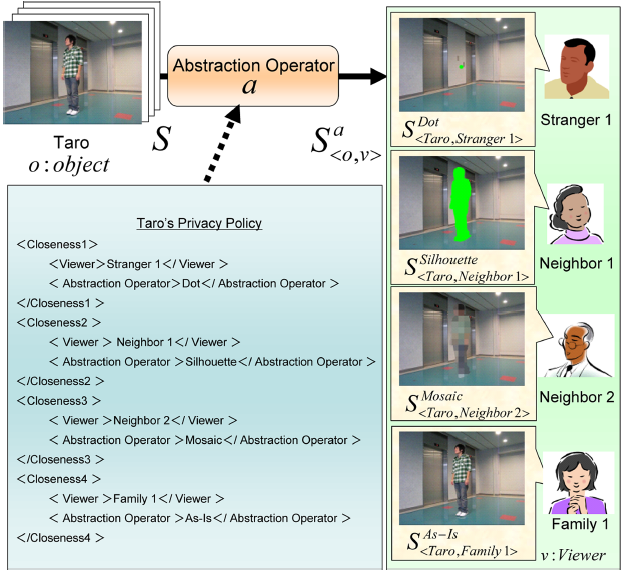
\includegraphics[width=.5\textwidth]{img//prisurv_simple_demo.png}}
\caption{PriSurv simple run case \cite{chinomi2008PriSurv}.}
\label{fig:prisurv}
\end{figure}
Figure~\ref{fig:prisurv2} shows the architecture of the PriSurv system. It consists of three main parts: Video Server, Main Server and Network. It also has six different components: \textbf{Analyzer}, \textbf{Profile Generator}, \textbf{Profile Base}, \textbf{Access Controller}, \textbf{Abstractor} and \textbf{Video Data Base}. 

The \textbf{Analyzer}, which is a part of the video server, is responsible for identifying different objects. Each identifiable object must have its own \ac{RFID}-tag. The surveillance area is divided into smaller N x N areas and the location area of each \ac{RFID}-tag is determined by an \ac{RFID}-reader. Each object inside the original image is extracted and then identified separately by comparing the obtained visual data with the binary images of each object. 

The \textbf{Profile Generator} is used for setting up privacy policies for different members of the system. Each member's personal information such as name, age, gender, address and privacy policy is stored securely inside the \textbf{Profile Base}. The Profile Generator is also responsible for converting data taken from the GUI to \ac{XML}-based syntax. The profile of each member can only be updated by them and other members have no access to this data. 

The \textbf{Access Controller} determines the closeness relationship between a requesting viewer and an object to be monitored by reading the \ac{XML}-based privacy policies of the object stored inside the Profile Base. Once the types of abstraction operators are extracted, the Access Controller sends them to the Abstractor. 

The \textbf{Abstractor} is an image processor that performs visual abstraction by using abstraction operators. 

The \textbf{Video Data Base} stores past video data and makes it available to viewers after appropriate visual abstractions are performed. 
\begin{figure}[t]
\centerline{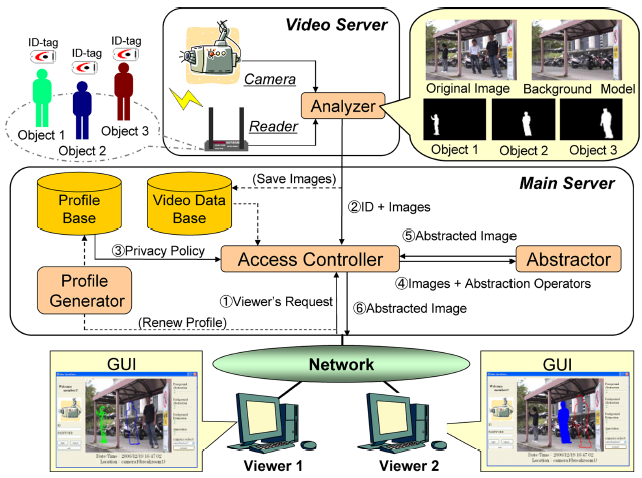
\includegraphics[width=.5\textwidth]{img//prisurv_arch.png}}
\caption{PriSurv system overview \cite{chinomi2008PriSurv}.}
\label{fig:prisurv2}
\end{figure}

\subsection{Cardea Framework}\label{Cardea}
As discussed in section \ref{Intro}, there have been several unfruitful past attempts at protecting visual privacy regarding the pervasiveness of cameras. The PriSurv system, which was discussed in the previous section, relies on extra facilities such as \ac{RFID}-tags and readers, similarly to other technologies. Thus, it is not a feasible solution for built-in cameras. 

The Cardea framework \cite{shu2016cardea} does not rely on such or similar extra facilities. Instead, it takes advantage of computer vision techniques, which are effective and reliable. Moreover, it allows people to change their privacy preferences dynamically, e.g. by using predefined hand gestures. The framework also specifies context elements, such as scenes and the presence of others. People can set their personal privacy profiles, the hand gestures to be recognised by cameras for flexible interactions, and their context related privacy preferences. For example, some people might prefer their visual appearance to be hidden inside bars, but not in parks. But in case they change their mind and, for example, decide to appear in a photo taken inside a bar, they can indicate it with a hand gesture. Devices using the framework will automatically compute factors related to the context, check people's privacy preferences, and protect their visual appearance by blurring their face.

\subsubsection{Key Concepts}
\begin{figure}[t]
\centerline{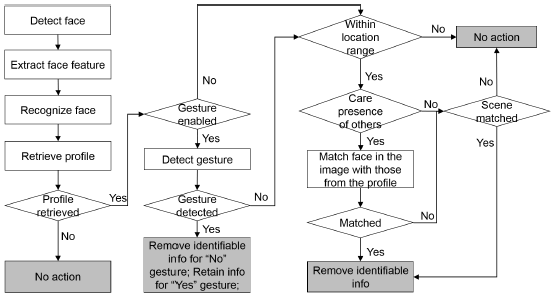
\includegraphics[width=.5\textwidth]{img/cardea_workflow.png}}
\caption{Cardea framework workflow \cite{shu2016cardea}.}
\label{fig:cardea}
\end{figure}

A few key concepts have to be briefly described before proceeding to the system overview. A person who has a device with an integrated camera and is taking photos is referred to as the \textbf{recorder}. People who may appear in these photos are the \textbf{bystanders}. Bystanders who do not want to be identifiable in the photos can express their privacy preferences by using the Cardea framework. On the other hand, the recorder who cares and respects the privacy preferences of the bystanders can use the Cardea framework to take photos. Both the recorder and the bystanders are classified as \textbf{users} of the Cardea privacy protection framework. Each bystander sets their \textbf{privacy profile}. Each profile contains information such as \textbf{context elements}, \textbf{gesture interaction} options, and the \textbf{privacy protection action} to be made. Bystanders have different privacy concerns depending on the context elements which can be locations, scenes and nearby people. The framework supports two gesture interactions: a victory sign and a palm, which stand for “Yes” and “No”, respectively, to the question “Would you like to appear in the taken photo?”. If a bystander does not use any of these gestures while the photo is taken, then the default privacy settings set in their privacy profile apply. The taken action in order to protect the visual privacy is face blurring. But further methods such as full body blurring, blending the body region into the background, or replacing the face with an average face are possible to be integrated. All of the bystanders' preferences are stored inside a \textbf{cloud} which accepts requests from the recorder and processes images in such way that the privacy preferences of the bystanders appearing in the images are respected. Figure~\ref{fig:cardea} visualizes the decision workflow of the Cardea framework. Decisions are made according to the computing results from the camera and remote cloud, then the original image is processed, in case it contradicts the privacy preferences of the bystanders. 

\subsubsection{System Overview}
\begin{figure}[t]
\centerline{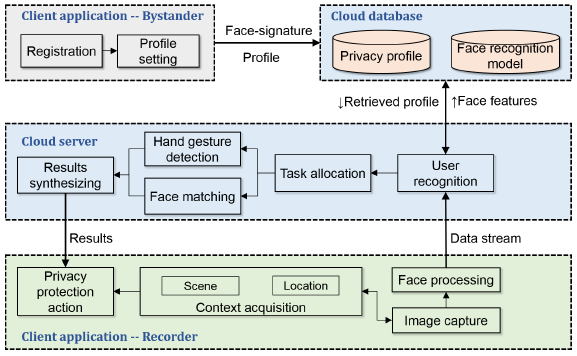
\includegraphics[width=.5\textwidth]{img/cardea_overview_diagram.png}}
\caption{Cardea framework system overview \cite{shu2016cardea}.}
\label{fig:cardea2}
\end{figure}

Figure~\ref{fig:cardea2} shows the interactions between the major components. Cardea is composed of the client app and the cloud server. Bystanders can register, setup their profile settings and upload their photo by using the user interface of the client application. The face features of the bystander are extracted and stored into the cloud server's database to be used for training the face recognition model. The privacy profile is also stored in the database. Bystanders can change their privacy preferences at any time later. 

Recorders use the client application to take photos. The application detects faces in the taken photos, extracts face features and computes context elements on the device. The face matching, user recognition and hand gesture detection processes are done on the cloud server, because they are computationally-intensive and infeasible on most devices. Once the results from the cloud are received, protection action will be performed. 

The cloud server is responsible for storing user profiles and processing detection tasks upon requests from the recorder side. The user recognition process is divided into three steps. The first step consists in detecting face regions on the image before filtering the results in order to reduce false positives. The second step is to extract face features in a compact, but still discriminative way, so the face detection is done using these features rather than comparing just raw pixels. The last step is to match these representative features to faces stored on the cloud database. 

The location filtering feature helps users defining specific locations in which they may worry more about their privacy. The location of the device taking a picture is obtained directly from the \ac{GPS}. Scene classification is a more complex concept, because it does not only rely to places, but also gives information about the current activities of people. The framework covers 9 general scene groups which are further divided into more specific scenes. In total, there are 98 different scenes. Users can more easily specify their privacy preferences by selecting from these general scene groups. 


\subsubsection{Example run case}
\begin{figure}[t]
\centerline{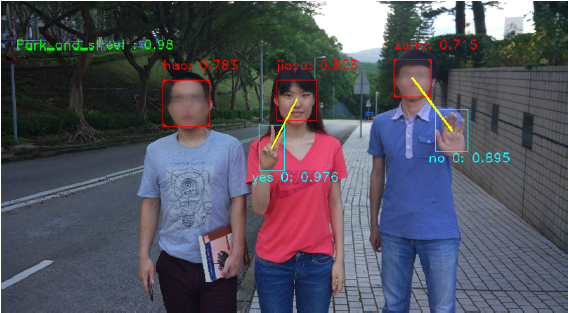
\includegraphics[width=.5\textwidth]{img/cardea_example.png}}
\caption{Cardea framework example run case \cite{shu2016cardea}.}
\label{fig:cardea3}
\end{figure}

Figure~\ref{fig:cardea3} shows a privacy protection example of the Cardea framework. The framework detects three registered users, two hand gestures and a scene. The scene is classified correctly as Park \& street. The face of Hao is detected and blurred by default in order to match his visual privacy preferences. The face of Zerry, under normal circumstances, would not have been blurred, but because he is doing a “No” gesture while this particular picture is taken, his face is blurred. Jiayu has the opposite case of Zerry. Under normal circumstances, her face would have been blurred, but because of her “Yes” gesture, her face is identifiable.


\subsection{ConsenShare}\label{ConsenShare}
Over the last decade, the sharing of varieties of \ac{IPD} and \ac{MSPD} online has drastically increased, due to emergence of \ac{OSN}s such as Facebook. The shared data can include very diverse content such as contact data, location data, multimedia data (audio, photo, video) and genomic data. Such data often involves information that is not only about the individual who shares them online, but also related to other data subjects \cite{ahern2007}. ConsenShare is a framework for ensuring the consent of bystanders when \ac{IPD} and \ac{MSPD} is about to be published online.

\subsubsection{ConsenShare Overview}
The ConsenShare framework \cite{olteanu2018consensual} considers three major entities: The users, the \ac{CMS} (e.g. OpenSNP for genomic data, Flickr for photos, or YouTube for videos) and the \ac{IMS} (responsible for identification of the users involved in the content). In practice, agencies or popular OSNs, such as Facebook, could play the role of the \ac{IMS}. Responsibility could be also split across several entities. Content uploaded to the CMS will be first sent for verification to all users whose privacy could be compromised, once identified by the \ac{IMS}. The users will also receive contextual information about the upload content, such as the identity of the uploader, target audience, upload time, etc. The content will be visible to the target audience only after it is confirmed by all the users. 

The developers of ConsenShare assume that the \ac{CMS} and \ac{IMS} are honest, trustable and independent parties. However, they could still be curious and try to infer sensitive information from the data observed. Moreover, conclusions about social ties among users could be made. For instance, if a user named Bob often accepts that another user Alice shares content regarding him, then they are likely good friends. Other threats such as the creation of fake profiles and taking the identity of another individual still remain. The developers also assume that secure two-way communication channels, typically over HTTPS, have been established between all entities. A malicious user might still try to gather data and monitor communications among the different entities in the framework. 

\begin{figure}[t]
\centerline{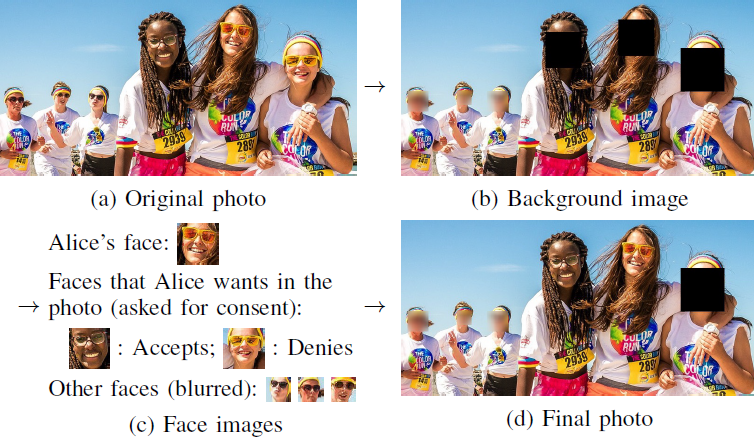
\includegraphics[width=.5\textwidth]{img/consen_example.png}}
\caption{ConsenShare framework example run case \cite{olteanu2018consensual}.}
\label{fig:consen}
\end{figure}
\subsubsection{Example run case}
Figure~\ref{fig:consen} shows an example application of the ConsenShare framework. (a) is the original photo taken by Alice. The application of Alice will produce the Background image (b) by removing the detected faces and extracting them into separate face images (c). The faces which appear in the background will be automatically blurred. The background and face images will be then sent to the \ac{CMS} and \ac{IMS}. The \ac{IMS} will identify two more individuals on the photo. They will receive a notification and will be asked for consent. After all users choose their privacy settings, the final photo (d) will be produced and hosted by the \ac{CMS}. In the example, one of the individuals accepts and the other one denies consent. Alice’s consent is automatically granted by default, as she is the photo’s uploader. 

\subsubsection{Possible extensions for ConsenShare}
The ConsenShare framework can be extended for other data, such as audio, video and co-location. Video and audio extensions are straightforward, because they are similar to the photo solution. The only difference is that the users have to be identified by the \ac{IMS} by using different solutions. Different solutions for identification in audio and video data have been proposed \cite{reynolds2002, mansour2015}. Co-location data privacy is a more complex topic, because the data itself can introduce dependencies among the different users. For example, if Alice and Bob appear in the same picture and they shared the location, it is uncertain how to protect the location data of their future posts. Alice’s future location posts could affect Bob’s location privacy and vice versa. 

\section{Limitations and challenges of privacy ensuring technologies}\label{Limitations}
Although the proposed technologies try to protect the privacy of bystanders, there are still some limitations and challenges. PriSurv, for example, relies on extra facilities: \ac{RFID}-tags and \ac{RFID}-readers \cite{chinomi2008PriSurv}. These requirements limit the efficiency of this framework for massive usage, because bystanders are not likely to wear such accessories (i.e. QR codes, colorful hats, etc.) in public places, according to Shu, Zheng and Hui~\cite{shu2016cardea}. Moreover, bystanders should not have to take action to protect their privacy nor actively pursue it as a goal~\cite{langheinrich2009privacy}. Therefore, relying on extra features is a limited approach in terms of usability and efficiency.  

The Cardea and ConsenShare frameworks are more feasible for massive usage. However, these frameworks have other challenges. Although the both frameworks have a good detection and matching rate of faces, there is still a small margin of false positives and false negatives. A false positive means that a face is detected in an area where none exists. A false negative, on the other hand, happens when an area containing a face is not detected. This case causes more privacy related problems, because a face appearing on a picture would never be protected. These challenges, however, should be overcome as technical progress in Machine Learning keeps raising and recognition algorithms get more and more perfected over time. 

All of the discussed technologies require creating a privacy profile and uploading private data to the system of the particular technology. This itself could be considered counter-productive, because users have to give out private data about themselves in order to protect their privacy, which includes this same data~\cite{denning2014situ}. Furthermore, the privacy of non-registered individuals is not taken into consideration. Only the ConsenShare framework is able to blur unrecognised individuals, but only if they appear in the background of a photo. Moreover, the proposed solutions are centralized. Maybe a decentralized peer-to-peer solution could potentially increase the trustfulness and make users more comfortable with sharing private data.

Above all, the main problem lies in the non-compulsory usage of these frameworks and their lack of regulation with laws. This means that, for now, only individuals that care for the privacy of others (or their own when they are bystanders to others) will likely bother using one of these technologies. As a result, this makes all the efforts made to ensure bystanders' privacy largely useless, since only a small portion of users would use such technologies from their own will; bystanders would remain unprotected from the majority of users and devices that are not privacy compliant. There could however be perspectives in solving this challenge: in~\cite{olteanu2018consensual}, the authors estimate that the use of systems that check for the consent of bystanders before online sharing could become mandatory by law in a few years. Still, as of now, and despite the good results these frameworks offer, none of them have gone outside the field of research, towards in-production, daily applications or devices.


\section{Conclusion}\label{Conclusion}
This report presented technologies that ensure the privacy of bystanders in various situations. An overview of past attempts at solving privacy issues has been seen, with the conclusion that they were mainly insufficient or inefficient. This leads back to tackling the problem today, with the challenge of providing flexible solutions for all users, depending on their placement on the privacy requirement spectrum. For this, modern technologies rely on user participation by asking users to create profiles with their personal privacy preferences. Some revolve around certain privacy threatening devices (e.g. drones, \ac{IoT} devices...)~\cite{yao2017privacy, bernd2020bystanders}, others are more generic (e.g. Cardea~\cite{shu2016cardea}). A distinction can be made between technologies that protect the privacy at time of data collection (e.g. when a picture or video is taken), and technologies that protect upon sharing of the data.

Several privacy enhancing tools have been presented. PrivSurv~\cite{chinomi2008PriSurv}, a video surveillance system, relies on  \ac{RFID} tags to detect individuals. It then processes the recorded videos accordingly to the privacy preferences defined by the concerned bystanders in the system's profile base: bystanders can choose between different abstraction operators that are selected by the access controller upon determination of the closeness between the bystander and the viewer. Despite not being the state of the art and relying on extra facilities, it remains an interesting first step and brings good ideas such as having profiles defined by the users themselves to match their personal requirements. 

The same idea was taken almost ten years later in Cardea \cite{shu2016cardea}, which is the second technology we presented. The strength of Cardea lies in the absence of external facilities: bystanders can indicate their consent for being photographed with simple hand gestures. The two client applications (i.e. one for the users that with to take pictures, the other for bystanders to register their privacy profile) are linked through the cloud server, where the resource-heavy calculations (i.e. user recognition, hand gesture detection) are performed. As a result, bystanders can easily manage their preferences, thanks to the scene management, their privacy profile, and the possibility of indicating a change in preferences with hand gestures. 

The third presented technology, ConsenShare~\cite{olteanu2018consensual}, takes a different approach for protecting bystanders' privacy. Instead of acting at the time of data collection, it monitors data where bystanders are involved and necessitates the consent of said bystanders before users are allowed to share the data. This approach gives control to bystanders who become systematically aware if content they appear on is planned to be published. This way, bystanders can not only control their visual privacy, but also their location privacy. This kind of system is critical to address big privacy and ethical issues where sensible aspects of bystanders are disclosed, such as revenge pornography. 

Despite our research, we could not find audio-centred technologies that aim to protect the privacy of bystanders, despite the existence for tools for protecting the audio privacy of users (e.g. in~\cite{larson2011accurate, ahmed2020preech}). This underlines the need for tools that aim to protect the audio privacy of bystanders. The same assessment is made for location, although it is mentioned in ConsenShare (regarding the sharing co-location).

One issue that remains, and is likely to stay until made mandatory by law, is that individuals are never required to use any of the proposed privacy enhancing tools. This means that bystanders' privacy can only be qualitative if a high number of users adopt these systems. Ideally, ubiquitous devices should have privacy by design, and bystanders should not have to take action to protect their privacy. Another limitation comes in the perception that creating privacy profiles on a cloud for ensuring one's own protection is a paradoxical, counter-productive action. Lastly, and more importantly, all of the presented technologies, although promising and efficient, stayed in the field of research. Privacy protection for bystanders is still not addressed in everyday-use end-user applications and devices, despite the growing interest in research. However, the growth of clouds facilitate solutions like Cardea, making the use of such tools in everyday life a hopefully soon reality.

\section*{Abbreviations and Acronyms}
\addcontentsline{toc}{section}{Abbreviations and Acronyms}
\begin{acronym}[Bash]
\acro{IoT} {\textit{Internet of Things}}
\acro{AR} {\textit{Augmented Reality}}
\acro{RFID} {\textit{Radio-frequency identification}}
\acro{XML} {\textit{Extensible Markup Language}}
\acro{GPS} {\textit{Global Positioning System}}
\acro{OSN} {\textit{Online Social Networks}}
\acro{MSPD} {\textit{Multiple-Subject Personal Data}}
\acro{IPD} {\textit{Interdependent Personal Data}}
\acro{CMS} {\textit{Content Management Service}}
\acro{IMS} {\textit{Identity Management Service}}
\end{acronym}

\printbibliography

\end{document}
